\chapter{Anwendbarkeit für die SAP Experience Garage Technology Plattform}

Inhalt dieses Kapitels ist eine Ausführung zur SAP Experience Garage Technology Plattform gefolgt von der Einschätzung bezüglich möglicher Implementierbarkeit des Konzepts
eines Learning-NFTs für die Plattform.
Dafür sollen die Relevanz der im vorigen Kapitel analysierten Aspekte des Learning-NFT in Gegenüberstellung mit dem Nutzen für Plattform und Benutzer und dem Implementierungsaufwand bewertet werden.

\section{Die SAP Experience Garage Technology Plattform}

Die SAP Experience Garage Technology Plattform ist eine \dq Gamified Collaboration and Microlearning Plattform\dq{}.
Sie ist also eine Lernplattform die kleine Lerneinheiten \dq spielerisch\dq{} und kollaborativ anbietet.
Angefangen mit der Vision einer kleinen Gruppe von SAP Mitarbeitern sich miteinander durch den Anwendungs-Dschungel bei SAP zu kämpfen entstand im Juli 2018 die Digital Heroes Community.
Seitdem entwickelt sich die Plattform stetig weiter und bietet mittlerweile unter dem Namen Experience Garage Technology Plattform neben Microlearnings zu Anwendungen wie Microsoft PowerPlattform, Jira und so weiter
auch diverse Inhalte zu Themen wie Diversity, Inclusive Leadership, 3D-Druck und vielen weiteren an.

Um ein Hero (so werden Benutzer der Plattform genannt) zu werden muss sich ein neuer Benutzer zuerst registrieren.
Danach stehen ihm alle Mircolearnings, welche auf der Plattform Missionen genannt werden, zur Verfügung.
Werden mehrere Missionen zu einem Thema angeboten werden sie zusätzlich in Tracks gruppiert.
Für abgeschlossene Missionen bekommt der Hero Punkte gutgeschrieben und kann Abzeichen bekommen.
Je nach Gesamtzahl der gesammelten Punkte wird der Hero dann auf ein bestimmtes Level gesetzt.
Angefangen beim Status Hero (50 Punkte) bis hin zu Wonder-Hero (3000 Punkte) kann dieses Level auf der Plattform von anderen Teilnehmern eingesehen werden (beispielsweise im Leaderboard) und sorgt für Vergleichbarkeit und spielerischen Wettkampf.

    \begin{figure}
        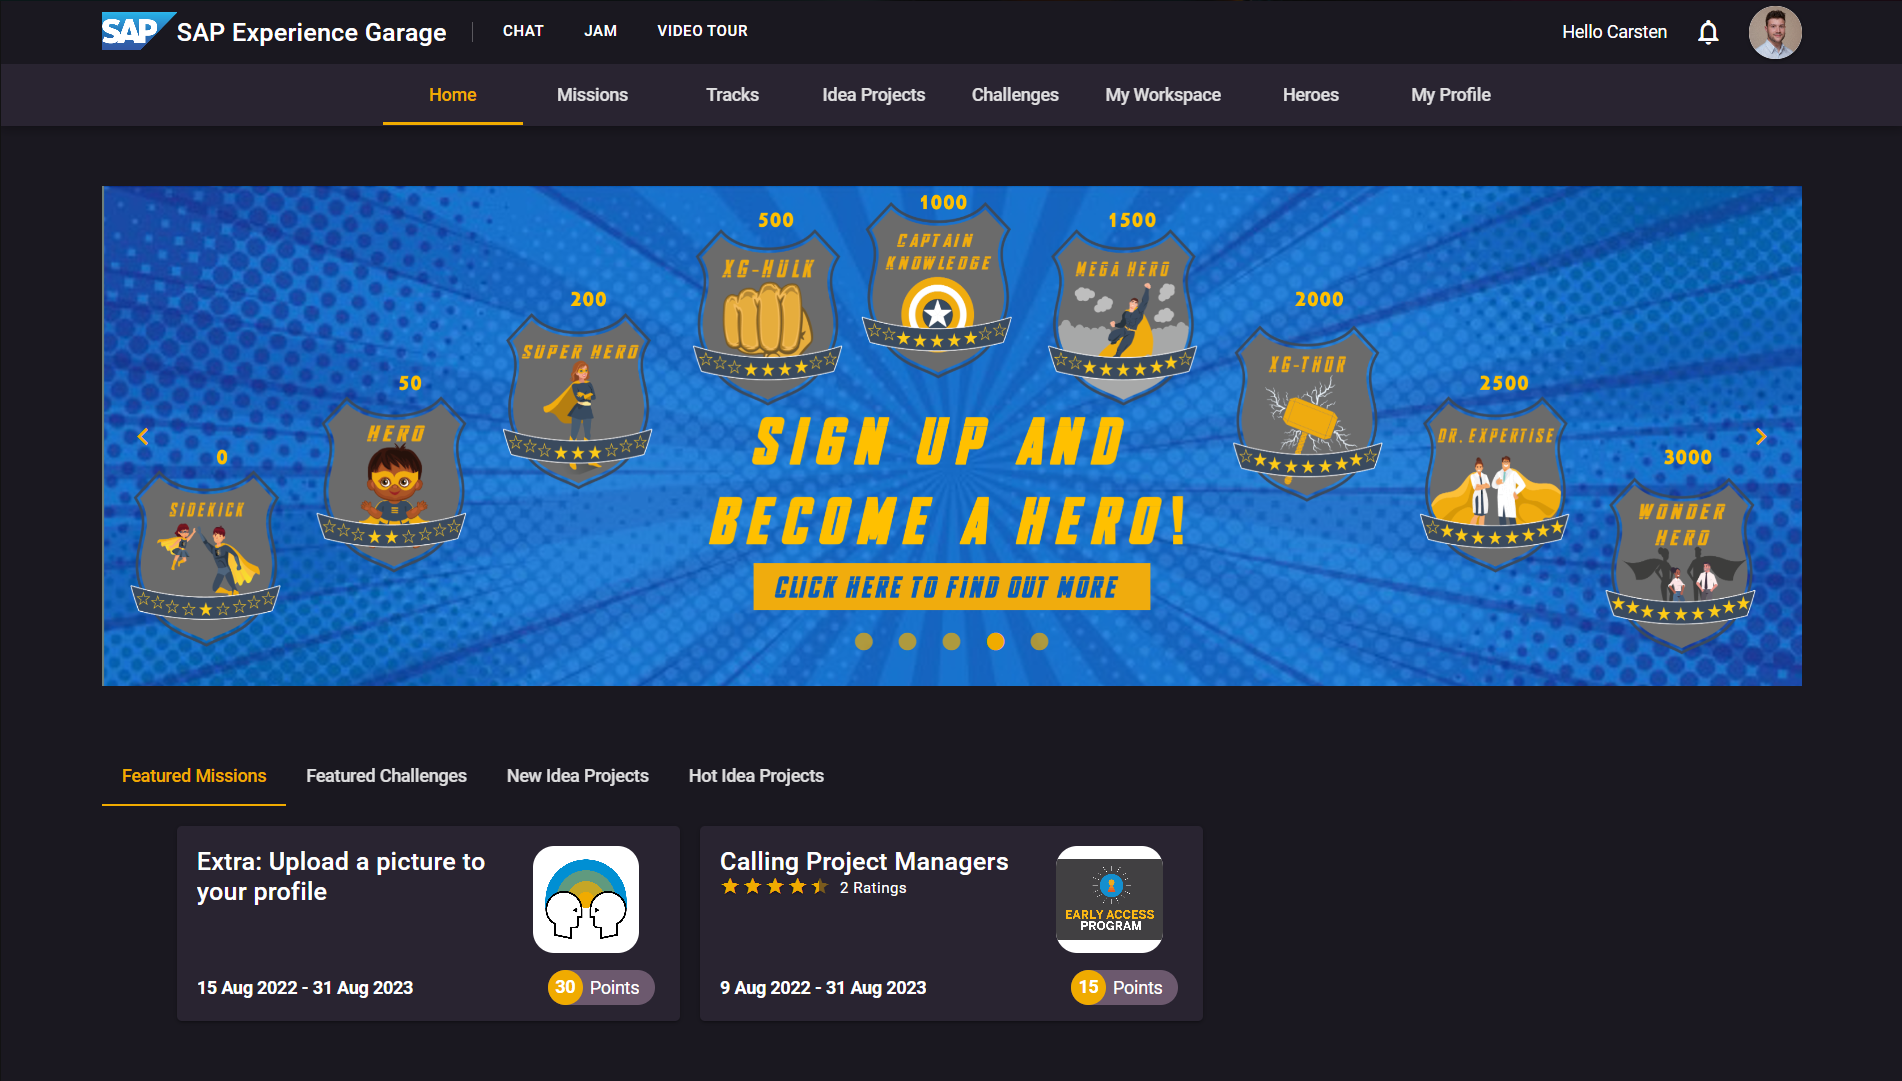
\includegraphics[width=15.8cm]{Bilder/XGTP.PNG}
        \centering
        \caption{Startseite der Experience Garage Plattform}
        \label{fig:xgtp}
    \end{figure}

\section{Anwendbarkeit des Learning-NFT für die Experience Garage Technology Plattform} \label{testref}

Besonders relevant am Konzept des dynamischen Learning-NFT ist die eingebaute Methode und Funktionsweise zum Lernen durch wiederholtes Beschäftigen mit dem Inhalt.
Dieses Wiederholen sorgt für deutlich nachhaltigere Lernerfolge und hilft die Auswirkungen der Vergessenskurve nach Ebbinghaus gering zu halten.
Abhängig davon, ob man dieser Lernmethode folgt, wird man dafür mit einer Anpassung des Scores belohnt beziehungsweise bestraft.
Lernt man nicht weiter und beschäftigt sich nicht weiterhin mit dem Thema, nimmt das Wissen des Teilnehmers ab, es verringert sich der Score.
Lernt der Teilnehmer weiter, bewahrt und baut er auf sein Wissen auf, steigt der Score.
Das sorgt für eine sinnvolle aktuelle Vergleichbarkeit und Qualifizierungsmöglichkeit. Der Wert hat also Relevanz.
Die Implementierung eines solchen Scores für verschiedene Wissensbereichen auf der Plattform wäre ähnlich zu dem bisherigen Punktesystem und könnte mit wenig Aufwand implementiert werden.

Weniger interessant für die SAP Experience Garage Technology Plattform ist das Thema Datenerhebung zum Lernverhalten.
Denn da die Plattform bereits eine Online-Anwendung ist, können bereits viele Daten zum Lernverhalten getrackt und erhoben werden.
Die Auswirkungen der Implementierung des Learning-NFT würden demnach diesbezüglich eher klein ausfallen.

Mögliche Verbesserungen in den Punkten Fälschungssicherheit und Transparenz sind in diesem Kontext für die Plattform auch eher weniger interessant.
Denn die angesprochene Fälschungssicherheit des NFT (siehe Kapitel \ref{fundt}) greift erst nach Validierung einer abgeschlossenen Lerneinheit.
Diese wird in den meisten Fällen vom Teilnehmer selbst und nur selten durch einen Admin vorgenommen.
Die Plattform vertraut von vornherein die Ehrlichkeit der Benutzer. Fälschungen können dann schon unkompliziert an dieser Stelle auftreten.
Die Fälschungssicherheit des Scores nach der Validierung ist also weniger relevant.
Zudem sind die gesammelten Punkte eines Teilnehmers für jeden Nutzer der Plattform einsehbar, womit bezogen auf Transparenz bereits ein Werkzeug der Kontrolle bereitsteht.

Der vielleicht interessanteste Aspekt des dynamischen Learning-NFT ist den Score in einem NFT abzulegen.
Auf der einen Seite wäre das eine sehr moderne Art der sicheren Speicherung und Learning-\ac{NFT} könnte vom Hype um die Technologie profitieren.
Auf der anderen Seite bietet der NFT-Ansatz kaum einen nennenswerten Vorteil.
Die Plattformunabhängigkeit als auch Fälschungssicherheit und Transparenz sind für unsere Plattform und deren Benutzer kaum bis nicht relevant.
Und die Methodik und Funktionsweise zum Lernen durch wiederholtes Beschäftigen in Verknüpfung mit einem Score lässt sich auch ohne einen NFT, dann als normaler Wert in einer Datenbank speichern.
Größtes Manko am NFT-Aspekt ist jedoch seine sehr aufwändige Implementierung. Es müsste eine komplette Side-Chain mit Verbindung zu einer Blockchain entwickelt werden. Das kostet viel Zeit und verursacht hohe Kosten.
Zudem würde jede Änderung des Scores eine Transaktion in der Side-Chain auslösen, die dann je nach Aufbau der Side-Chain, gesammelte Transaktionen in einer Root-Transaktion an die Root-Chain weitergibt.
Jede dieser Transaktionen würde nach heutigem Stand 1.67 US-Dollar kosten, im Vergleich zu einem weiteren Wert in der Datenbank ein immenser Kostenunterschied \parencite[vgl.][]{Redaktion.04.07.2022}.
